\title{Unoffical notes: Search for boosted top+Higgs resonance in the all hadronic decay mode}
\author{Lucas Corcodilos}
\date{\today}

\documentclass[10pt]{article}
\usepackage[margin=0.5in]{geometry}
\usepackage{graphicx}
\usepackage{url}
\usepackage{float}
\restylefloat{table}

\begin{document}
\maketitle
\section{Analysis strategy and selection}

Dijet search for boosted $X \to tH$. The benchmark, $X$, is a VLQ $T'$ produced
in association with a bottom quark. The interaction with an associated top quark
is currently ignored since the simulation samples are inconsistent with the UL
versions available for all other simulation. The associated quark will have 
much lower transverse momentum than the T' decay products and so the affect on
the analysis is expected to be small (ie. quark will be along beamline).

\subsection{Selection}
\begin{table}[H]
    \centering
    \begin{tabular}{|c |c |c |c|}
        \hline
        Signal region (SR) & QCD control for SR & Validation region (VR) & QCD control for VR \\
        \hline
        \multicolumn{4}{|c|}{Two AK8 jets separated by $\Delta \phi > \pi/2$} \\
        \multicolumn{4}{|c|}{$p_T > 350$ GeV for each jet} \\
        \multicolumn{4}{|c|}{$|\eta| < 2.4$ for each jet} \\
        \multicolumn{4}{|c|}{$m_{\mathrm{jet}} > 50$ for each jet} \\
        \hline
        \multicolumn{2}{|c|}{At least one jet top tagged} & \multicolumn{2}{|c|}{No jet top tagged} \\
        \hline
        \multicolumn{1}{|c|}{Higgs tag pass} & \multicolumn{1}{|c|}{Higgs tag fail} & \multicolumn{1}{|c|}{Higgs tag pass} & \multicolumn{1}{|c|}{Higgs tag fail} \\
        \hline
    \end{tabular} 
    \label{table:selection}
    \caption{Analysis selection for four selection regions. A ``top tag'' refers to a selection of 
    a tagger score at least 0.632 and $105 < m_{\mathrm{jet}} < 210$ GeV, where the tagger could be DeepAK8
    or ParticleNet (see Section~\ref{sec:jets}). A ``Higgs tag'' refers to a tagger score selection of
    at least 0.9, where the tagger could be DeepAK8 or ParticleNet.}       
\end{table}

\section{Initial studies on jet tagging}
\label{sec:jets}
Two neural network based taggers are considered for jet tagging -
DeepAK8 and ParticleNet. Several aspects of these taggers can affect this
analysis and are considered when choosing between the taggers.

First and most importantly, the tagger must be decorrelated from the jet
mass so as not to sculpt the jet mass distribution. The two dimensional background
estimation method uses the jet mass as one of the axis in which to measure data.
If the taggers sculpt the jet mass so as to create a signal-like peak, the background
will be harder to discriminant from potential signal.

Additionally, the data-driven
estimate of the QCD multijet background relies on a smooth ratio of the distributions
of those events passing and failing the tagger. If the ``pass'' is sculpted and the ``fail''
is not, we cannot hope to use our transfer function method without introducing method
for potential signal bias.

Second, the tagger should be good at distinguishing between top and Higgs jets so the
tagger can be used to easily identify which side of the event is which physics object.
In particular, the analysis would benefit from a tagger that correctly identifes that 
real Higgs jets are not top jets.

Finally, the tagger should be efficient at removing background without requiring a 
MC-to-data scale factor that is large or has large uncertainties that could dominant
the total systematic uncertainty for the analysis.

With these three items in mind, we examined two variables - the difference in mass
between the two jets and the difference in top tagging scores between the two jets
- and plotted them against each other. In addition to considering the two taggers,
we also considered four scenarios based on the simulation truth.

From left to right in Figs. \ref{figs:DeepAK8_diff_2D} and \ref{figs:PN_diff_2D}:
\begin{itemize}
    \item The first scenario does nothing with simulation truth.
    \item The second scenario examines when neither the top nor Higgs jet identified by the
          tagger were able to be matched to their respective generator particle (``Bad match'').
    \item The third scenario examines when both the top and Higgs jets identified by the tagger
          were matched successfully to their respective generator particle (``Good match'').
    \item The fourth scenario identifies the top and Higgs jets based on the generator particle
          information and then the variables plotted are calculated based on this information.
\end{itemize}

In other words, the fourth scenario flips the order of operations of the third scenario.
The distributions for both taggers and the four scenarios are shown in Figs.
\ref{figs:DeepAK8_diff_2D} and \ref{figs:PN_diff_2D} where a 2016 $T' \to tH$ signal with
a $T'$ mass of 1200 GeV is examined.

\begin{figure}
    \centering
    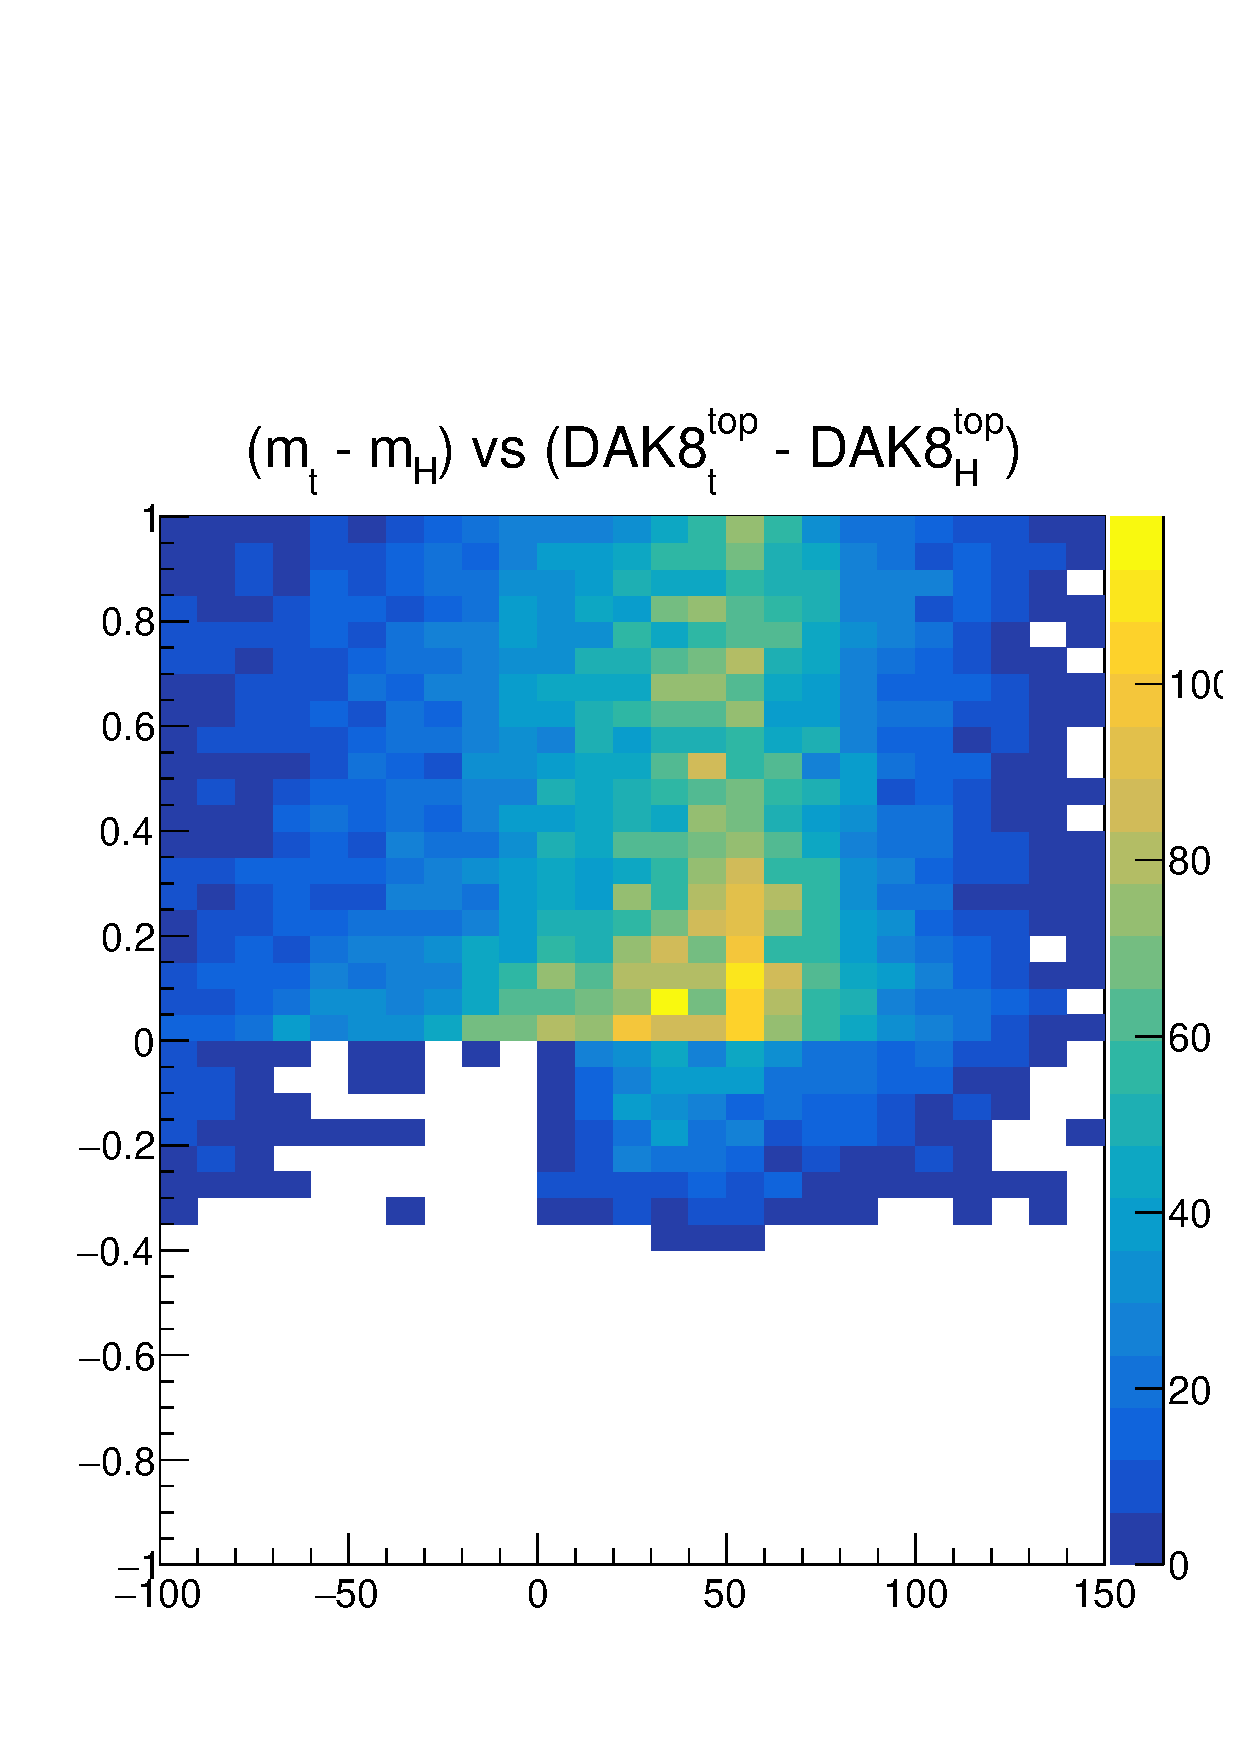
\includegraphics[page=1,width=0.24\textwidth]{../plots/diff2Dstudy.pdf}
    \includegraphics[page=2,width=0.24\textwidth]{../plots/diff2Dstudy.pdf}
    \includegraphics[page=3,width=0.24\textwidth]{../plots/diff2Dstudy.pdf}
    \includegraphics[page=4,width=0.24\textwidth]{../plots/diff2Dstudy.pdf}
    \caption{DeepAK8 studies}
    \label{figs:DeepAK8_diff_2D}
\end{figure}

\begin{figure}
    \centering
    \includegraphics[page=5,width=0.24\textwidth]{../plots/diff2Dstudy.pdf}
    \includegraphics[page=6,width=0.24\textwidth]{../plots/diff2Dstudy.pdf}
    \includegraphics[page=7,width=0.24\textwidth]{../plots/diff2Dstudy.pdf}
    \includegraphics[page=8,width=0.24\textwidth]{../plots/diff2Dstudy.pdf}
    \caption{ParticleNet studies}
    \label{figs:PN_diff_2D}
\end{figure}

\section{Kinematic distributions}

We further investigate kinematic variables which may be useful in increasing
the signal to background ratio in the analysis. Figures \ref{figs:pt} and 
\label{figs:etaY} compare simulation for all of Run 2.

\begin{figure}
    \includegraphics[width=0.32\textwidth]{../plots/pt0_Run2.pdf}
    \includegraphics[width=0.32\textwidth]{../plots/pt1_Run2.pdf}
    \includegraphics[width=0.32\textwidth]{../plots/HT_Run2.pdf}
    \label{figs:pt}
    \caption{The $p_T$ of the leading (left) and subleading (middle) jet in the event and the scalar sum of the two (right).
    The total background is represented as a stack of QCD (yellow) and ttbar (red) MC and the total is normalized to
    unity. The signal (black line) is separately normalized to unity.}
\end{figure}

\begin{figure}
    \includegraphics[width=0.49\textwidth]{../plots/deltaEta_Run2.pdf}
    \includegraphics[width=0.49\textwidth]{../plots/deltaY_Run2.pdf}
    \label{figs:etaY}
    \caption{The $|\Delta \eta|$ between the two candidate jets in the event. The total background
    is represented as a stack of QCD (yellow) and ttbar (red) MC and the total is normalized to
    unity. The signal (black line) is separately normalized to unity.}
\end{figure}


\section{Jet tagging variables}

Two variables are used to tag a canidate jet - the tagger score and the jet mass.
In order to inspect these variables, a series of N-1 plots are made - one for each
the top jet mass, top jet tagger score, Higgs jet mass, and Higgs jet tagger score.
When one variable is plotted, the other three are cut on.

Since this means a Higgs and top cannot be identified without impacting the distributions,
the top quark is assumed to be the leading jet in $p_T$. The MC truth shows this is true 50\%
of the time. The other N-1 cuts in a given plot should kill most
of the mis-matched events (where the top jet is actually a Higgs and vice versa)
with some fraction remaining. As can be seen in \ref{figs:DeepAK8_diff_2D}, that 
fraction is decently large when tagging a
real Higgs with the DeepAK8 top tagger. This effect explains the Higgs peak
in Figure \ref{figs:jetMassDAK8}.

Figures \ref{figs:jetMassDAK8}, \ref{figs:jetMassPN}, \ref{figs:jetDAK8}, and \ref{figs:jetPN}
compare simulation for all of Run 2.

\begin{figure}
    \includegraphics[width=0.49\textwidth]{../plots/mH_deepTagMD_cut_nminus1_Run2.pdf}
    \includegraphics[width=0.49\textwidth]{../plots/mt_deepTagMD_cut_nminus1_Run2.pdf}
    \label{figs:jetMassDAK8}
    \caption{Shape comparison of the jet mass distributions for the Higgs (left) and top (right) jets
    when using the mass decorrelated DeepAK8 tagger. The total background
    is represented as a stack of QCD (yellow) and ttbar (red) MC and the total is normalized to
    unity. The signal (black line) is separately normalized to unity.}
\end{figure}

\begin{figure}
    \includegraphics[width=0.49\textwidth]{../plots/mH_particleNet_cut_nminus1_Run2.pdf}
    \includegraphics[width=0.49\textwidth]{../plots/mt_particleNet_cut_nminus1_Run2.pdf}
    \label{figs:jetMassPN}
    \caption{Shape comparison of the jet mass distributions for the Higgs (left) and top (right) jets
    when using the ParticleNet tagger (not mass decorrelated). The total background
    is represented as a stack of QCD (yellow) and ttbar (red) MC and the total is normalized to
    unity. The signal (black line) is separately normalized to unity.}
\end{figure}

\begin{figure}
    \includegraphics[width=0.49\textwidth]{../plots/deepTagMD_H_cut_nminus1_Run2.pdf}
    \includegraphics[width=0.49\textwidth]{../plots/deepTagMD_top_cut_nminus1_Run2.pdf}
    \label{figs:jetDAK8}
    \caption{Shape comparison of the DeepAK8 score distributions for the Higgs (left) and top (right) jets
    when using the mass decorrelated DeepAK8 tagger. The total background
    is represented as a stack of QCD (yellow) and ttbar (red) MC and the total is normalized to
    unity. The signal (black line) is separately normalized to unity.}
\end{figure}

\begin{figure}
    \includegraphics[width=0.49\textwidth]{../plots/particleNet_H_cut_nminus1_Run2.pdf}
    \includegraphics[width=0.49\textwidth]{../plots/particleNet_top_cut_nminus1_Run2.pdf}
    \label{figs:jetPN}
    \caption{Shape comparison of the ParticleNet score distributions for the Higgs (left) and top (right) jets
    when using the mass decorrelated ParticleNet tagger. The total background
    is represented as a stack of QCD (yellow) and ttbar (red) MC and the total is normalized to
    unity. The signal (black line) is separately normalized to unity.}
\end{figure}

\section{Blinded fits to data}

\section{Data and simulation samples}

\begin{center}
    \begin{tabular}{l p{40em}}
        \multicolumn{2}{c}{2016} \\
        \hline
        \multicolumn{1}{c}{Setname} & \multicolumn{1}{c}{DAS location} \\
        \hline
        TprimeB 800 GeV & \path{/TprimeBToTH_M-800_LH_TuneCP5_PSweights_13TeV-madgraph_pythia8/RunIISummer19UL16NanoAODv2-106X_mcRun2_asymptotic_v15-v1/NANOAODSIM} \\
        TprimeB 900 GeV & \path{/TprimeBToTH_M-900_LH_TuneCP5_PSweights_13TeV-madgraph_pythia8/RunIISummer19UL16NanoAODv2-106X_mcRun2_asymptotic_v15-v1/NANOAODSIM} \\
        TprimeB 1000 GeV & \path{/TprimeBToTH_M-1000_LH_TuneCP5_PSweights_13TeV-madgraph_pythia8/RunIISummer19UL16NanoAODv2-106X_mcRun2_asymptotic_v15-v1/NANOAODSIM} \\
        TprimeB 1100 GeV & \path{/TprimeBToTH_M-1100_LH_TuneCP5_PSweights_13TeV-madgraph_pythia8/RunIISummer19UL16NanoAODv2-106X_mcRun2_asymptotic_v15-v1/NANOAODSIM} \\
        TprimeB 1200 GeV & \path{/TprimeBToTH_M-1200_LH_TuneCP5_PSweights_13TeV-madgraph_pythia8/RunIISummer19UL16NanoAODv2-106X_mcRun2_asymptotic_v15-v1/NANOAODSIM} \\
        TprimeB 1300 GeV & \path{/TprimeBToTH_M-1300_LH_TuneCP5_PSweights_13TeV-madgraph_pythia8/RunIISummer19UL16NanoAODv2-106X_mcRun2_asymptotic_v15-v1/NANOAODSIM} \\
        TprimeB 1400 GeV & \path{/TprimeBToTH_M-1400_LH_TuneCP5_PSweights_13TeV-madgraph_pythia8/RunIISummer19UL16NanoAODv2-106X_mcRun2_asymptotic_v15-v1/NANOAODSIM} \\
        TprimeB 1500 GeV & \path{/TprimeBToTH_M-1500_LH_TuneCP5_PSweights_13TeV-madgraph_pythia8/RunIISummer19UL16NanoAODv2-106X_mcRun2_asymptotic_v15-v1/NANOAODSIM} \\
        TprimeB 1600 GeV & \path{/TprimeBToTH_M-1600_LH_TuneCP5_PSweights_13TeV-madgraph_pythia8/RunIISummer19UL16NanoAODv2-106X_mcRun2_asymptotic_v15-v1/NANOAODSIM} \\
        TprimeB 1700 GeV & \path{/TprimeBToTH_M-1700_LH_TuneCP5_PSweights_13TeV-madgraph_pythia8/RunIISummer19UL16NanoAODv2-106X_mcRun2_asymptotic_v15-v1/NANOAODSIM} \\
        TprimeB 1800 GeV & \path{/TprimeBToTH_M-1800_LH_TuneCP5_PSweights_13TeV-madgraph_pythia8/RunIISummer19UL16NanoAODv2-106X_mcRun2_asymptotic_v15-v1/NANOAODSIM} \\
        ttbar-allhad & \path{/TTToHadronic_TuneCP5_13TeV-powheg-pythia8/RunIISummer19UL16NanoAODv2-106X_mcRun2_asymptotic_v15-v1/NANOAODSIM} \\
        ttbar-semilep & \path{/TTToSemiLeptonic_TuneCP5_13TeV-powheg-pythia8/RunIISummer19UL16NanoAODv2-106X_mcRun2_asymptotic_v15-v1/NANOAODSIM} \\
        QCDHT700 & \path{/QCD_HT700to1000_TuneCP5_PSWeights_13TeV-madgraphMLM-pythia8/RunIISummer19UL16NanoAODv2-106X_mcRun2_asymptotic_v15-v1/NANOAODSIM} \\
        QCDHT1000 & \path{/QCD_HT1000to1500_TuneCP5_PSWeights_13TeV-madgraphMLM-pythia8/RunIISummer19UL16NanoAODv2-106X_mcRun2_asymptotic_v15-v1/NANOAODSIM} \\
        QCDHT1500 & \path{/QCD_HT1500to2000_TuneCP5_PSWeights_13TeV-madgraphMLM-pythia8/RunIISummer19UL16NanoAODv2-106X_mcRun2_asymptotic_v15-v1/NANOAODSIM} \\
        QCDHT2000 & \path{/QCD_HT2000toInf_TuneCP5_PSWeights_13TeV-madgraphMLM-pythia8/RunIISummer19UL16NanoAODv2-106X_mcRun2_asymptotic_v15-v1/NANOAODSIM} \\
        DataB1 & \path{/JetHT/Run2016B-ver1_HIPM_UL2016_MiniAODv1_NanoAODv2-v1/NANOAOD} \\
        DataB2 & \path{/JetHT/Run2016B-ver2_HIPM_UL2016_MiniAODv1_NanoAODv2-v1/NANOAOD} \\
        DataC & \path{/JetHT/Run2016C-UL2016_MiniAODv1_NanoAODv2-v1/NANOAOD} \\
        DataD & \path{/JetHT/Run2016D-UL2016_MiniAODv1_NanoAODv2-v1/NANOAOD} \\
        DataE & \path{/JetHT/Run2016E-UL2016_MiniAODv1_NanoAODv2-v1/NANOAOD} \\
        DataF & \path{/JetHT/Run2016F-UL2016_MiniAODv1_NanoAODv2-v2/NANOAOD} \\
        DataG & \path{/JetHT/Run2016G-UL2016_MiniAODv1_NanoAODv2-v1/NANOAOD} \\
        DataH & \path{/JetHT/Run2016H-UL2016_MiniAODv1_NanoAODv2-v1/NANOAOD} \\
    \end{tabular}
\end{center}

\begin{center}
    \begin{tabular}{l p{40em}}
        \multicolumn{2}{c}{2017} \\
        \hline
        \multicolumn{1}{c}{Setname} & \multicolumn{1}{c}{DAS location} \\
        \hline
        TprimeB 800 GeV & \path{/TprimeBToTH_M-800_LH_TuneCP5_PSweights_13TeV-madgraph_pythia8/RunIISummer19UL17NanoAODv2-106X_mc2017_realistic_v8-v1/NANOAODSIM} \\
        TprimeB 900 GeV & \path{/TprimeBToTH_M-900_LH_TuneCP5_PSweights_13TeV-madgraph_pythia8/RunIISummer19UL17NanoAODv2-106X_mc2017_realistic_v8-v1/NANOAODSIM} \\
        TprimeB 1000 GeV & \path{/TprimeBToTH_M-1000_LH_TuneCP5_PSweights_13TeV-madgraph_pythia8/RunIISummer19UL17NanoAODv2-106X_mc2017_realistic_v8-v1/NANOAODSIM} \\
        TprimeB 1100 GeV & \path{/TprimeBToTH_M-1100_LH_TuneCP5_PSweights_13TeV-madgraph_pythia8/RunIISummer19UL17NanoAODv2-106X_mc2017_realistic_v8-v1/NANOAODSIM} \\
        TprimeB 1200 GeV & \path{/TprimeBToTH_M-1200_LH_TuneCP5_PSweights_13TeV-madgraph_pythia8/RunIISummer19UL17NanoAODv2-106X_mc2017_realistic_v8-v1/NANOAODSIM} \\
        TprimeB 1300 GeV & \path{/TprimeBToTH_M-1300_LH_TuneCP5_PSweights_13TeV-madgraph_pythia8/RunIISummer19UL17NanoAODv2-106X_mc2017_realistic_v8-v1/NANOAODSIM} \\
        TprimeB 1400 GeV & \path{/TprimeBToTH_M-1400_LH_TuneCP5_PSweights_13TeV-madgraph_pythia8/RunIISummer19UL17NanoAODv2-106X_mc2017_realistic_v8-v1/NANOAODSIM} \\
        TprimeB 1500 GeV & \path{/TprimeBToTH_M-1500_LH_TuneCP5_PSweights_13TeV-madgraph_pythia8/RunIISummer19UL17NanoAODv2-106X_mc2017_realistic_v8-v1/NANOAODSIM} \\
        TprimeB 1600 GeV & \path{/TprimeBToTH_M-1600_LH_TuneCP5_PSweights_13TeV-madgraph_pythia8/RunIISummer19UL17NanoAODv2-106X_mc2017_realistic_v8-v1/NANOAODSIM} \\
        TprimeB 1700 GeV & \path{/TprimeBToTH_M-1700_LH_TuneCP5_PSweights_13TeV-madgraph_pythia8/RunIISummer19UL17NanoAODv2-106X_mc2017_realistic_v8-v1/NANOAODSIM} \\
        TprimeB 1800 GeV & \path{/TprimeBToTH_M-1800_LH_TuneCP5_PSweights_13TeV-madgraph_pythia8/RunIISummer19UL17NanoAODv2-106X_mc2017_realistic_v8-v1/NANOAODSIM} \\
        ttbar-allhad & \path{/TTToHadronic_TuneCP5_13TeV-powheg-pythia8/RunIISummer19UL17NanoAODv2-106X_mc2017_realistic_v8-v1/NANOAODSIM} \\
        ttbar-semilep & \path{/TTToSemiLeptonic_TuneCP5_13TeV-powheg-pythia8/RunIISummer19UL17NanoAODv2-106X_mc2017_realistic_v8-v1/NANOAODSIM} \\
        QCDHT700 & \path{/QCD_HT700to1000_TuneCP5_PSWeights_13TeV-madgraphMLM-pythia8/RunIISummer19UL17NanoAODv2-106X_mc2017_realistic_v8-v1/NANOAODSIM} \\
        QCDHT1000 & \path{/QCD_HT1000to1500_TuneCP5_PSWeights_13TeV-madgraphMLM-pythia8/RunIISummer19UL17NanoAODv2-106X_mc2017_realistic_v8-v1/NANOAODSIM} \\
        QCDHT1500 & \path{/QCD_HT1500to2000_TuneCP5_PSWeights_13TeV-madgraphMLM-pythia8/RunIISummer19UL17NanoAODv2-106X_mc2017_realistic_v8-v1/NANOAODSIM} \\
        QCDHT2000 & \path{/QCD_HT2000toInf_TuneCP5_PSWeights_13TeV-madgraphMLM-pythia8/RunIISummer19UL17NanoAODv2-106X_mc2017_realistic_v8-v1/NANOAODSIM} \\
        DataB & \path{/JetHT/Run2017B-UL2017_MiniAODv1_NanoAODv2-v1/NANOAOD} \\
        DataC & \path{/JetHT/Run2017C-UL2017_MiniAODv1_NanoAODv2-v1/NANOAOD} \\
        DataD & \path{/JetHT/Run2017D-UL2017_MiniAODv1_NanoAODv2-v1/NANOAOD} \\
        DataE & \path{/JetHT/Run2017E-UL2017_MiniAODv1_NanoAODv2-v1/NANOAOD} \\
        DataF & \path{/JetHT/Run2017F-UL2017_MiniAODv1_NanoAODv2-v2/NANOAOD} \\
    \end{tabular}
\end{center}

\begin{center}
    \begin{tabular}{l p{40em}}
        \multicolumn{2}{c}{2018} \\
        \hline
        \multicolumn{1}{c}{Setname} & \multicolumn{1}{c}{DAS location} \\
        \hline
        TprimeB 800 GeV & \path{/TprimeBToTH_M-800_LH_TuneCP5_PSweights_13TeV-madgraph_pythia8/RunIISummer19UL18NanoAODv2-106X_upgrade2018_realistic_v15_L1v1-v1/NANOAODSIM} \\
        TprimeB 900 GeV & \path{/TprimeBToTH_M-900_LH_TuneCP5_PSweights_13TeV-madgraph_pythia8/RunIISummer19UL18NanoAODv2-106X_upgrade2018_realistic_v15_L1v1-v1/NANOAODSIM} \\
        TprimeB 1000 GeV & \path{/TprimeBToTH_M-1000_LH_TuneCP5_PSweights_13TeV-madgraph_pythia8/RunIISummer19UL18NanoAODv2-106X_upgrade2018_realistic_v15_L1v1-v1/NANOAODSIM} \\
        TprimeB 1100 GeV & \path{/TprimeBToTH_M-1100_LH_TuneCP5_PSweights_13TeV-madgraph_pythia8/RunIISummer19UL18NanoAODv2-106X_upgrade2018_realistic_v15_L1v1-v1/NANOAODSIM} \\
        TprimeB 1200 GeV & \path{/TprimeBToTH_M-1200_LH_TuneCP5_PSweights_13TeV-madgraph_pythia8/RunIISummer19UL18NanoAODv2-106X_upgrade2018_realistic_v15_L1v1-v1/NANOAODSIM} \\
        TprimeB 1300 GeV & \path{/TprimeBToTH_M-1300_LH_TuneCP5_PSweights_13TeV-madgraph_pythia8/RunIISummer19UL18NanoAODv2-106X_upgrade2018_realistic_v15_L1v1-v1/NANOAODSIM} \\
        TprimeB 1400 GeV & \path{/TprimeBToTH_M-1400_LH_TuneCP5_PSweights_13TeV-madgraph_pythia8/RunIISummer19UL18NanoAODv2-106X_upgrade2018_realistic_v15_L1v1-v1/NANOAODSIM} \\
        TprimeB 1500 GeV & \path{/TprimeBToTH_M-1500_LH_TuneCP5_PSweights_13TeV-madgraph_pythia8/RunIISummer19UL18NanoAODv2-106X_upgrade2018_realistic_v15_L1v1-v1/NANOAODSIM} \\
        TprimeB 1600 GeV & \path{/TprimeBToTH_M-1600_LH_TuneCP5_PSweights_13TeV-madgraph_pythia8/RunIISummer19UL18NanoAODv2-106X_upgrade2018_realistic_v15_L1v1-v1/NANOAODSIM} \\
        TprimeB 1700 GeV & \path{/TprimeBToTH_M-1700_LH_TuneCP5_PSweights_13TeV-madgraph_pythia8/RunIISummer19UL18NanoAODv2-106X_upgrade2018_realistic_v15_L1v1-v1/NANOAODSIM} \\
        TprimeB 1800 GeV & \path{/TprimeBToTH_M-1800_LH_TuneCP5_PSweights_13TeV-madgraph_pythia8/RunIISummer19UL18NanoAODv2-106X_upgrade2018_realistic_v15_L1v1-v1/NANOAODSIM} \\
        ttbar-allhad & \path{/TTToHadronic_TuneCP5_13TeV-powheg-pythia8/RunIISummer19UL18NanoAODv2-106X_upgrade2018_realistic_v15_L1v1-v1/NANOAODSIM} \\
        ttbar-semilep & \path{/TTToSemiLeptonic_TuneCP5_13TeV-powheg-pythia8/RunIISummer19UL18NanoAODv2-106X_upgrade2018_realistic_v15_L1v1-v1/NANOAODSIM} \\
        QCDHT700 & \path{/QCD_HT700to1000_TuneCP5_PSWeights_13TeV-madgraphMLM-pythia8/RunIISummer19UL18NanoAODv2-106X_upgrade2018_realistic_v15_L1v1-v1/NANOAODSIM} \\
        QCDHT1000 & \path{/QCD_HT1000to1500_TuneCP5_PSWeights_13TeV-madgraphMLM-pythia8/RunIISummer19UL18NanoAODv2-106X_upgrade2018_realistic_v15_L1v1-v1/NANOAODSIM} \\
        QCDHT1500 & \path{/QCD_HT1500to2000_TuneCP5_PSWeights_13TeV-madgraphMLM-pythia8/RunIISummer19UL18NanoAODv2-106X_upgrade2018_realistic_v15_L1v1-v1/NANOAODSIM} \\
        QCDHT2000 & \path{/QCD_HT2000toInf_TuneCP5_PSWeights_13TeV-madgraphMLM-pythia8/RunIISummer19UL18NanoAODv2-106X_upgrade2018_realistic_v15_L1v1-v1/NANOAODSIM} \\
        DataA & \path{/JetHT/Run2018A-UL2018_MiniAODv1_NanoAODv2-v1/NANOAOD} \\
        DataB & \path{/JetHT/Run2018B-UL2018_MiniAODv1_NanoAODv2-v1/NANOAOD} \\
        DataC & \path{/JetHT/Run2018C-UL2018_MiniAODv1_NanoAODv2-v1/NANOAOD} \\
        DataD & \path{/JetHT/Run2018D-UL2018_MiniAODv1_NanoAODv2-v1/NANOAOD} \\
    \end{tabular}
\end{center}

\end{document}